\section{Related Work and Preliminaries}
\label{sec:related_prelim}
We discuss related work and preliminaries for our core application, sequence generative modeling; see \Cref{app:extended_related} for further literature review.

Our method unifies two perspectives on sequence modeling:  Bayesian filtering along the time axis, denoted by subscript $t$, and diffusion along an ``uncertainty'' (or noise level) axis denoted by superscript $k$. In the following, we denote observations as $\bx \in \mathcal{X}$ and latent states as $\bz \in \mathcal Z$. 

\paragraph{Bayesian Filtering.}
Given a Hidden Markov Model (HMM) defined by latent states $\mathbf{z}_t$ and observations $\bx_t$, a Bayes filter is a probabilistic method for estimating latent states recursively over time from incoming observations. A prior model $p(\mathbf{z}_{t+1}|\mathbf{z}_{t})$ infers a belief over the next state given only the current state, and an observation model infers a belief over the next observation given the current latent state $p(\bx_{t}|\mathbf{z}_{t})$. When a new observation is made, a posterior model $p(\mathbf{z}_{t+1}|\mathbf{z}_{t}, \bx_{t+1})$ provides an updated estimation of the next latent state $\mathbf{z}_{t+1}$. When trained end-to-end with neural networks \cite{dreamer,planet}, latent states are not an estimate of any physical quantity, but a sufficiently expressive latent that summarizes past observations for predicting future observations $(\bx_{t'})_{t'>t}$ in the sequence. 

\begin{figure*}[t]
    \centering
    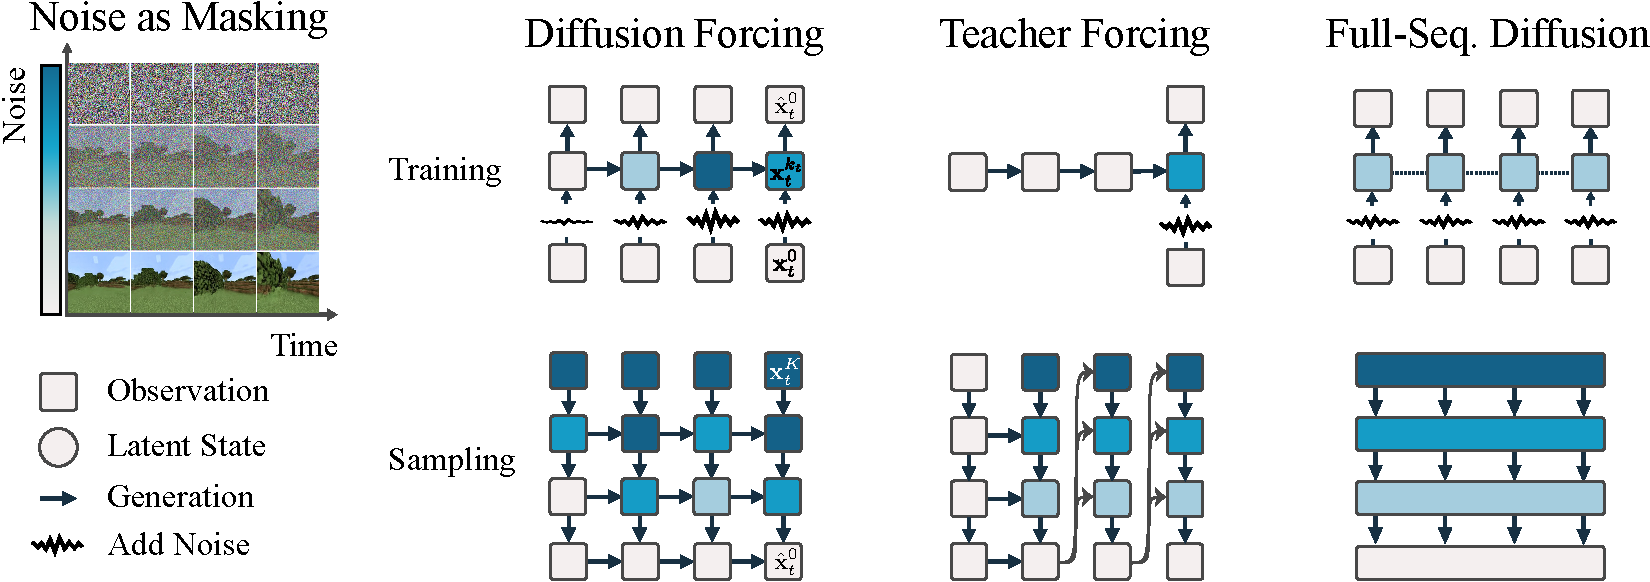
\includegraphics[width=\linewidth]{figures/pdf/Overview_best_guess.pdf}
    \caption{\textbf{Method Overview.} 
    Diffusion Forcing trains causal sequence neural networks (such as an RNN or a masked transformer) to denoise flexible-length sequences where each frame of the sequence can have a \emph{different} noise level.
    In contrast, next-token prediction models, common in language modeling, are trained to predict a single next token from a \emph{ground-truth} sequence (teacher forcing~\cite{teacher_forcing}), and full-sequence diffusion, common in video generation, train non-causal architectures to denoise all frames in a sequence at once with the \emph{same} noise level.
    \algo{} thus \emph{interleaves} the time axis of the sequence and the noise axis of diffusion, unifying strengths of both alternatives and enabling completely new capabilities (see Secs.~\ref{sec:zigzag_example},\ref{sec:method_decision_making}).
    }
    \label{fig:method}
    \vspace{-5pt}
\end{figure*}


\newcommand{\eye}{\mathbf{I}}

\newcommand{\bmu}{\bm{\mu}}
\newcommand{\beps}{\bm{\epsilon}}
\paragraph{Diffusion Models.}
Diffusion models~\cite{sohl2015deep,ho2020denoising} have proven to be highly expressive and reliable generative models.
We review their essentials here. Let $q(\bx)$ denote a data distribution of interest, and let $\bx^0 \equiv \bx \sim q$. We consider a forward diffusion process that gradually adds Gaussian noise to a data point over a series of time steps. This process is modeled as a Markov chain, where the data at each step \( k \) is noised incrementally:
\begin{equation}
    \label{eqn:forward_diffusion}
    q(\bx^k|\bx^{k-1}) = \mathcal{N}(\bx^k; \sqrt{1-\beta_k}\bx^{k-1}, \beta_k \mathbf{I})
\end{equation}
where \( \mathcal{N} \) is the normal distribution and \( \beta_k \) is the variance of the noise added at each step controlled by a schedule $\{\beta_k \in (0, 1)\}_{k=1}^K$. The process continues until the data is converted into pure noise at \( \bx^K \).
The reverse process is also a Markov chain and attempts to recreate the original data from the noise with a parameterized model $p_\theta$:
\begin{equation}
    p_\theta(\bx^{k-1}|\bx^k) = \mathcal{N}(\bx^{k-1}; \bmu(\bx^k, k), \gamma_k \eye),
\end{equation}
where the mean $\bmu$ is a model with a neural network, and where it is shown~\cite{ddpm} that one can set the covariance to the identity scaled by a fixed constant $\gamma_k$  depending on $k$. Adopting the standard exposition, we reparametrize the mean $\bmu$ in terms of noise prediction $\beps = (\sqrt{1-\bar{\alpha}_t})^{-1}\xtk-\sqrt{\bar{\alpha}_t} \bmu$. This leads \cite{ho2020denoising}  to the following least squares objective: 
\begin{equation}
    \mathcal{L}(\theta) = \mathbb{E}_{k, \bx^0, \epsilon}\left[\| \beps^k - \beps_\theta(\bx^k, k) \|^2\right],
\end{equation}
where $\bx^k = \sqrt{\bar{\alpha_t}}\bx^0 +  \sqrt{1-\bar{\alpha_t}}\epsilon^k$ and $\beps^k \sim \cN(0,\mathbf{I})$ . One can then sample from this model via Langevin dynamics $\bx^{k-1} \gets \frac{1}{\sqrt{\alpha_k}}(\bx_t^{k} - \frac{1-\alpha_k}{\sqrt{1-\bar{\alpha}_k}}\beps_{\theta}(\bx_t^{k},k) + \sigma_k \mathbf{w})$ ~\cite{ho2020denoising}. 

\paragraph{Guidance of Diffusion Models.}
Guidance~\cite{ho2022classifierfree,dhariwal2021diffusion} allows biasing diffusion generation towards desirable predictions at sampling time. 
We focus on classifier guidance~\cite{dhariwal2021diffusion}: given a classifier $c(y|\bx^k)$ of some desired $y$ (e.g. class or success indicator), one modifies the Langevin sampling ~\cite{ddpm} gradient $\beps_\theta(\bx^k, k)$ to be $\beps_\theta(\bx^k, k)-\sqrt{1-\bar{\alpha}_k}\nabla_{x^k}\log c(y|\bx^k)$. This allows sampling from the joint distribution of $\bx$ and class label $y$ without the need to train a conditional model. Other energies such as a least-squares objective comparing the model output to a desirable ground truth have been explored in applications such as decision making~\cite{dhariwal2021diffusion,janner2022planning}.

\paragraph{Next-Token Prediction Models.}
Next-token prediction models are sequence models that predict the next frame $\bx_{t+1}$ given past frames $\bx_{1:t}$. At training time, one feeds a neural network with $\bx_{1:t}$ and minimizes $||\hat{\bx}-\bx||^2$ for continuous data or a cross-entropy loss for discrete data~\cite{teacher_forcing}. At sampling time, one samples the next frame $\hat{\bx}_{t+1}$ following $p(\bx_{t+1}|\bx_{1:t})$. If one treats $\hat{\bx}_{t+1}$ as $\bx_{t+1}$, one can use the same model to predict $\bx_{t+2}$ and repeat until a full sequence is sampled. Unlike full-sequence diffusion models, next-token models do not accept multi-step guidance, as prior frames must be fully determined to sample future frames. 

\paragraph{Diffusion Sequence Models.}
Diffusion has been widely used in sequence modeling. \cite{li2022diffusionlm} use full-sequence diffusion models to achieve controllable text generation via guidance, such as generating text following specified parts of speech.  \cite{ho2022video} trains full-sequence diffusion models to synthesize short videos and uses a sliding window to roll out longer conditioned on previously generated frames. \cite{janner2022planning} uses full-sequence diffusion models as planners in offline reinforcement learning. This is achieved by training on a dataset of interaction trajectories with the environment and using classifier guidance at sampling time to sample trajectories with high rewards towards a chosen goal. \cite{rasul2021autoregressive} modifies auto-regressive models to denoise the next token conditioned on previous tokens. It trains with teacher forcing~\cite{teacher_forcing} and samples next-token auto-regressively for time series data. Most similar to our work is AR-Diffusion \cite{wu2023ardiffusion}, which trains full-sequence text diffusion with a causal architecture with linearly dependent noise level along the time axis. We provide a detailed comparision between this approach and ours  in \Cref{app:extended_related}.

